In order to assess nonnative pronunciation a machine learning system was chosen as solution.
In this section we will review the way the system works and explain the concepts 
and techiniques required to build it.

~

\begin{figure}[H]
	\centering
	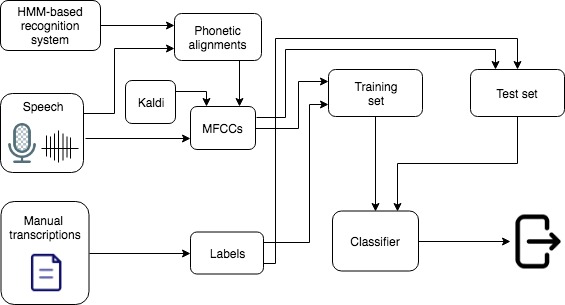
\includegraphics[width=0.8\textwidth]{files/figures/method/general-structure.jpg}
	\caption{General System Architecture}
	\label{fig:methodGeneralArchitecture}
\end{figure}

Given a phone utterance the objective is to determine wheter or not it was correctly
pronounced, with the possibility of returning
a more specific value that measures how well or bad that uttered phone
was pronounced.

The input data consists of recordings of read
speech that belongs to nonnative speakers with different proficiency levels.
The phone is the unit of analysis, so the first step is extracting the information
for each phone instance in the utterances.  In order to do so,
an HMM-based (Hidden Markov Model) recognition system is used to obtain the phonetic
segmentations of the utterances, and these segmentations along with an external tool
called \emph{Kaldi} are then used to extract the 
acoustic features for each phone. At the same time, manual transcriptions of profesional
annotators are used to obtain labels for each instance. A label has two possible values (0 or 1),
and determines if a given instance of a phone was correctly or incorrectly pronounced.

After that, labels and features are used to prepare a dataset: training and test sets. The first
one is used to explore different models and find the best configurations. 
After chosing the final solution, the hypothesis is tested against the test set 
and the results are analyzed.

